%Перечня рецензируемых научных изданий
\subsection*{\Large Общая характеристика работы}
\fontsize{14pt}{15pt}\selectfont
\subsubsection*{\large{Актуальность темы исследования}}

Взаимодействие различных компонент приложений часто реализуется с помощью встроенных языков, то есть приложение, созданное на одном языке, генерирует код на другом языке и передаёт этот код на выполнение в соответствующее окружение. Примерами могут служить динамические SQL-запросы к базам данных в Java-коде или формирование HTML-страниц в PHP-приложениях. Генерируемая программа собирается таким образом, чтобы в момент выполнения результирующий фрагмент кода (строка) представлял собой корректное выражение на соответствующем языке. Такой подход весьма гибок, так как позволяет использовать для формирования таких фрагментов кода различные строковые операции (replace, substring и т.д.) и комбинировать код из различных источников (например, учитывать текстовый ввод пользователя, что часто используется для задания фильтров при конструировании SQL-запросов). Необходимо отметить, что такой подход не имеет дополнительных накладных расходов, присущих, например, ORM-технологиям, и это позволяет достигать высокую производительность. 

Однако динамическое формирование программ часто происходит с помощью операций конкатенации в циклах, условных операторах или рекурсивных процедурах, что приводит к множеству возможных вариантов значений для каждого выражения в момент выполнения. При этом фрагменты кода на встроенных языках воспринимаются компилятором исходного языка как простые строки, не подлежащие дополнительному анализу, что приводит к высокой вероятности возникновения ошибок во время выполнения программы. В худшем случае такие ошибки не приведут к прекращению работы приложения, что явно указало бы на проблему, но целостность данных при этом может оказаться нарушенной. Более того, например, при наличии в коде приложения встроенных SQL-запросов нельзя, не проанализировав все динамически формируемые выражения, точно ответить на вопрос о том, с какими элементами базы данных не взаимодействует система, и  удалить их. При переносе такой системы на другую СУБД необходимо гарантировать, что для всех динамически формируемых выражений значение в момент выполнения будет корректным кодом на языке новой СУБД. Кроме того, при создании приложений распространённой практикой является использование интегрированных сред разработки, производящих подсветку синтаксиса и автодополнение, сигнализирующих о синтаксических ошибках, предоставляющих возможность рефакторинга. Всё это значительно упрощает процесс разработки и отладки приложений и полезно не только для основного языка, но и для встроенных языков. Для решения данных задач необходимы инструменты, проводящие статический анализ динамически формируемых программ.  

\subsubsection*{\large{Степень разработанности темы исследования}}

Анализу динамически формируемых строковых выражений посвящены работы таких зарубежных учёных как Кюнг-Гу Дох (Kyung-Goo Doh), Ясухико Минамиде (Minamide Yasuhiko), Андерс Мёллер (Anders M{\o}ller), а также отечественных учёных --- А.А.~Бреслава и М.Д.~Шапот. Вопросы проверки корректности динамически формируемых выражений достаточно хорошо изучены, однако актуальным представляется проведение более сложных видов статического анализа, требующих построения структурного представления динамически формируемого кода. То есть требуется механизм синтаксического анализа динамически формируемых выражений, позволяющий строить лес вывода для всех возможных значений соответствующего выражения. 

Методы обобщённого синтаксического анализа, использованные в данной работы, изложены в трудах таких учёных как Масару Томита (Masaru Tomita), Элизабет Скотт (Elizabeth Scott) и Адриан Джонстон (Adrian Johnstone) из университета Royal Holloway (Великобритания), Ян Рекерс (Jan Rekers, University of Amsterdam), Элко Виссер (Eelco Visser) и других.

Так же важной является разработка компонентов, упрощающих создание новых инструментов для решения конкретных задач. Данных подход хорошо исследован в области разработки компиляторов, где широкое распространение получили генераторы анализаторов и пакеты стандартных библиотек. 

В работах отечественных учёных С.Л.~Трошина, М.Д.~Шапот и Э.В.~Попова, а так же зарубежных учёных Антони Клеви (Anthony Cleve), Жан-Люк Эно (Jean-Luc Hainaut), Йост Виссер (Joost Visser) и других рассматриваются различные аспекты реинжиниринга систем, использующих встроенные SQL-запросы, однако не формулируется общего метода реинжиниринга таких систем. Разработка такого метода является актуальной задачей.

Существует также ряд инструментов для работы с динамически формируемыми выражениями: Alvor и IntelliLang, предоставляющие поддержку встроенных языков в интегрированных средах разработки, JSA и PHPSA, позволяющие искать ошибки в выражениях на встроенных языках, SQLWays, поддерживающий трансформацию выражений на встроенных языках, SAFELI --- инструмент статического анализа, предназначенный для определения возможности SQL-инъекций в Web-приложениях и некоторые другие. Однако, эти инструменты имеют существенные ограничения по функциональности: они не поддерживают часто встречающиеся на практике сложные способы формирования строковых выражений (ветвления, циклы) и решают, как правило, только одну узкую задачу (например, проверку корректности или поиск уязвимых конструкций).

Таким образом, актуальной является задача дальнейшего исследования синтаксического анализа динамически формируемых строковых выражений, а так же возможностей построения структурного представления динамически формируемого кода. Кроме этого важным является решение вопросов практического применения средств анализа динамически формируемого кода: упрощение разработки инструментов анализа и создание методов их применения в реинжиниринге программного обеспечения.

\subsubsection*{\large{Объект исследования}}

 Объектом исследования являются методы, алгоритмы и программные средства обработки динамически формируемых программ, а также задача реинжиниринга информационных систем.

\subsubsection*{\large{Цель и задачи диссертационной работы}}

\textbf{Целью} данной работы является создание комплексного подхода к статическому синтаксическому анализу динамически формируемых программ.

Для достижения поставленной цели сформулированы следующие \textbf{задачи}.
\begin{enumerate}
    \item Разработать алгоритм синтаксического анализа динамически формируемых программ, позволяющий обрабатывать регулярную аппроксимацию множества значений выражения в точке выполнения гарантирующий конечность представления леса вывода.
    \item Разработать архитектуру инструментария для разработки программных средств статического анализа динамически формируемых строковых выражений.
    \item Разработать метод анализа и обработки встроенного программного кода в проектах по реинжинирингу информационных систем.
\end{enumerate}

Цели и задачи диссертационной работы соответствуют области исследований паспорта специальности 05.13.11 ``Математическое и программное обеспечение вычислительных машин, комплексов и компьютерных сетей'' --- пункту 
1 (модели, методы и алгоритмы проектирования и анализа программ и программных систем, их эквивалентных преобразований, верификации и тестирования),
пункту 2 (языки программирования и системы программирования, семантика программ) и пункту 10 (оценка качества, стандартизация и сопровождение программных систем).

\subsubsection*{\large{Методология и методы исследования}}

Методология исследования основана на подходе к спецификации и анализу формальных языков, который начал активно развиваться в 50-х годах 20-го века при изучении естественных языков (работы Н. Хомского). В последствии этот подход получил широкое распространение в областях, связанных с обработкой языков программирования.
При этом основными элементами данного подхода являются алфавит и грамматика исследуемого языка, разбиение автоматической обработки языка на выполнение таких шагов, как лексический, синтаксический и семантический анализ. Решаемые в связи с этим задачи связаны с поиском эффективных алгоритмов, выполняющих эти шаги. 

В работе применяется алгоритм обобщённого восходящего синтаксического анализа RNGLR, созданный Элизабет Скотт (Elizabeth Scott) и Адриан Джонстон (Adrian Johnstone) из университета Royal Holloway (Великобритания). Для компактного хранения леса вывода использовалась структура данных Shared Packed Parse Forest (SPPF), которую предложил Ян Рекерс (Jan Rekers, University of Amsterdam). Доказательство завершаемости и корректности предложенного алгоритма проводилось с применением теории формальных языков, теории графов и теории сложности алгоритмов. Приближение множества значений динамически формируемого выражения строилось в виде регулярного множества, описываемого с помощью конечного автомата.

\subsubsection*{\large{Положения, выносимые на защиту}}
\begin{enumerate}
    \item Разработан алгоритм синтаксического анализа динамически формируемых выражений, позволяющий обрабатывать произвольную регулярную аппроксимацию множества значений выражения в точке выполнения, реализующий 
    эффективное управление стеком и гарантирующий конечность представления леса вывода. Доказана завершаемость и корректность предложенного алгоритма при анализе регулярной аппроксимации, представимой в виде произвольного конечного автомата без $\varepsilon$-переходов. 
    \item Создана архитектура инструментария для разработки программных средств статического анализа динамически формируемых строковых выражений.
    \item Разработан метод анализа и обработки встроенного программного кода в проектах по реинжинирингу информационных систем. 
\end{enumerate}


\subsubsection*{\large{Научная новизна}}

Научная новизна полученных в ходе исследования результатов заключается в следующем.

\begin{enumerate}

\item Алгоритм, предложенный в диссертации, отличается от аналогов (работы Андрея Бреслава, Кюнг-Гу Дох, Ясухико Минамиде) возможностью построения компактной структуры данных, 
содержащей деревья вывода для всех корректных генерируемых цепочек. Это позволяет как проверять корректность анализируемых выражений, так и проводить более сложные виды анализа, используя деревья вывода, 
хранящиеся в построенной структуре данных. Многие из существующих алгоритмов предназначены только для проверки корректности 
выражений, основанной на решении задачи о включении одного языка в другой (JSA, PHPSA). Выполнение более сложных видов анализа, трансформаций или построения леса разбора не предполагается. 

\item Новизна представленной архитектуры заключается в том, что она позволяет создать платформу для разработки инструментов, решающих широкий круг задач анализа динамически формируемого кода. Архитектуры готовых инструментов для анализа динамически формируемых строковых выражений (JSA, PHPSA, Alvor, Varis) ориентированы на решение конкретных задач для определённых языков программирования. Решение новых задач или поддержка других языков с помощью этих инструментов затруднены ввиду ограничений, накладываемых архитектурой и возможностями используемого алгоритма анализа. 

\item Метод анализа и обработки встроенного программного кода в проектах по реинжинирингу информационных систем предложен впервые. Существующие методы реинжиниринга не учитывают встроенный программный код, а работы, например, М.Д.~Шапот, Э.В.~Попова, А. Клеви, посвящены решению конкретных задач, не предлагают единого метода обработки встроенного программного кода.

\end{enumerate}

\subsubsection*{\large{Теоретическая и практическая значимость работы}}

Теоретическая значимость диссертационного исследования заключается в разработке формального алгоритма синтаксического анализа динамически формируемого кода, решающего задачу построения конечного представления леса вывода, не решаемую ранее, а также в формальном доказательстве завершаемости и корректности разработанного алгоритма. 

На основе полученных в работе научных результатов был разработан инструментарий (Software Development Kit, SDK), предназначенный для создания средств статического анализа динамически формируемых выражений. Данный инструментарий позволяет автоматизировать создание лексических и синтаксических анализаторов при разработке программных средств для решения задач реинжиниринга --- изучения и инвентаризации систем, автоматизации трансформации выражений на встроенных языках. Также данный инструментарий может использоваться при реализации поддержки встроенных языков в интегрированных средах разработки.

С использованием разработанного инструментария было реализовано расширение к инструменту ReSharper (ООО ``ИнтеллиДжей Лабс'', Россия), предоставляющее поддержку встроенного T-SQL в проектах на языке программирования C\# в среде разработки Microsoft Visual Studio. Так же было выполнено внедрение результатов работы в промышленный проект по переносу хранимого SQL-кода с MS-SQL Server 2005 на Oraclе 11gR2 (ЗАО ``Ланит-Терком'', Россия). 


\subsubsection*{\large{Степень достоверности и апробация результатов}}

Достоверность и обоснованность результатов исследования опирается на использование формальных методов исследуемой области, выполнение формальных доказательств и инженерные эксперименты.

Основные результаты работы были доложены на ряде международных научных конференциях: SECR-2012, SECR-2013, SECR-2014, TMPA-2014, Parsing@SLE-2013, рабочем семинаре ``Наукоемкое программное обеспечение'' при конференции PSI-2014. Доклад на конференции SECR-2014 был награждён премией Бертрана Мейера за лучшую исследовательскую работу в области программной инженерии. Разработка инструментальных средств на основе предложенного алгоритма была поддержана Фондом содействия развитию малых форм предприятий в технической сфере (программа УМНИК, проект \textnumero~162ГУ1/2013 и проект \textnumero~5609ГУ1/2014).

\subsubsection*{\large{Публикации по теме диссертации}}

Результаты диссертации изложены в 7 научных работах из которых 3~\cite{1,2,3} опубликованы в журналах из перечня рецензируемых научных изданий, 1~\cite{4} индексируются Scopus. Работы~\cite{1, 2, 3, 4, 5, 6, 7} написаны в соавторстве. В~\cite{1} С. Григорьеву принадлежит реализация ядра платформы YaccConstructor. В~\cite{2, 3} и~\cite{5} С. Григорьеву принадлежит постановка задачи, формулирование требований к разрабатываемым инструментальным средствам, работа над текстом. В~\cite{4} автору принадлежит идея исследования, реализация и описание алгоритма анализа встроенных языков на основе RNGLR-алгоритма.  В~\cite{6} С. Григорьеву принадлежит реализация инструментальных средств, проведение экспериментов, работа над текстом. В работе~\cite{7} автору принадлежит разработка алгоритма синтаксического анализа динамически формируемого кода.


\subsubsection*{\large{Объем и структура работы}}
Диссертация состоит из~введения, шести глав, заключения и~списка литературы. Полный объем диссертации \textbf{128}~страниц текста с~\textbf{26}~рисунками и~\textbf{8}~таблицами. Список литературы содержит \textbf{95}~наименований.

\subsection*{\Large Содержание работы}
Во \underline{\textbf{введении}} обосновывается актуальность исследований, выполненных в рамках данной диссертационной работы, приводится обзор научной литературы по изучаемой проблеме, формулируется цель, 
ставятся задачи работы, описывается научная новизна и практическая значимость представляемой работы.


В \underline{\textbf{первой главе}} проводится обзор области исследования. Рассматриваются подходы к анализу динамически формируемых строковых выражений и соответствующие инструменты. Описывается алгоритм обобщённого восходящего синтаксического анализа RNGLR, использованный в работе. Также описываются 
проекты YaccConstructor и ReSharper SDK, использованные в качестве технологий реализации результатов диссертации. На основе проведённого обзора можно сделать следующие выводы.

\begin{itemize}
    \item Проблема анализа строковых выражений актуальна в нескольких областях: поддержка встроенных языков в интегрированных средах разработки; оценка качества кода, содержащего динамически формируемые строковые выражения; реинжиниринг программного обеспечения.
    \item Большинство существующих технологических средств поддерживают конкретный внешний и встроенный языки и, как правило, решают только одну задачу (например, поиск ошибок). При этом, они плохо расширяемы, как в смысле поддержки других языков, так и в смысле решения новых задач. Полноценные средства разработки инструментов статического анализа динамически формируемых выражений, упрощающие создание решений для новых языков, отсутствуют.
    \item Для эффективного решения задач анализа строковых выражений необходимо структурное представление динамически формируемого кода, однако на текущий момент отсутствует законченное решение, позволяющего строить деревья вывода для динамически формируемых выражений.
\end{itemize}

Во \underline{\textbf{второй главе}} задача синтаксического анализа динамически формируемых выражений формализуется следующим образом: \textit{ для данной однозначной контекстно-свободной грамматики $G = \langle T, N, P, S \rangle$ и детерминированного конечного автомата без $\varepsilon$-переходов $M=(Q,\Sigma,\delta,q_0,q_f)$ такого, что $\Sigma \subseteq T$, необходимо построить конечную структуру данных $F$, содержащую деревья вывода в $G$ всех цепочек $\omega \in L(M)$, корректных относительно грамматики $G$, и не содержащую других деревьев. } Иными словами, необходимо построить алгоритм $\mathbb{P}$ такой, что
    $$(\forall \omega \in L(M)) (\omega \in L(G) \Rightarrow (\exists t \in \mathbb{P}(L(M),G))AST(t, \omega, G))$$
    $$\land (\forall t \in \mathbb{P}(L(M),G))(\exists \omega \in L(M))AST(t,\omega,G).$$ 
    Здесь $AST(t,\omega,G)$ --- это предикат, который истинен, если $t$ является деревом вывода $\omega$ в грамматике $G$.


Так как $\mathbb{P}$ игнорирует ошибки, то будем называть его алгоритмом \textit{ослабленного} (relaxed) синтаксического анализа регулярной аппроксимации динамически формируемого выражения.

Далее описывается алгоритм, решающий поставленную задачу: алгоритм синтаксического анализа регулярного множества на основе RNGLR, строящий конечную структуру данных, содержащую деревья вывода для 
всех цепочек анализируемого множества. Далее доказывается ряд вспомогательных утверждений, необходимых для доказательства основных утверждений о корректности предложенного алгоритма.

\textsc{Определение 1.} 
\emph{Корректное дерево}~--- это упорядоченное дерево со следующими свойствами.
\begin{enumerate}
  \item Корень дерева соответствует стартовому нетерминалу грамматики $G$.
  \item Листья соответствуют терминалам грамматики $G$. Упорядоченная последовательность листьев соответствует некоторому пути во входном графе.
  \item Внутренние узлы соответствуют нетерминалам грамматики $G$. Дети внутреннего узла (для нетерминала $N$) соответствуют символам правой части некоторой продукции для $N$ в грамматике $G$.
\end{enumerate}

\textsc{Лемма.}
\textit{Пусть задан внутренний граф $\mathcal{G}=(V,E)$. Тогда для каждого ребра GSS $(v_{t}, v_{h})$ такого, что $v_{t} \in V_{t}.processed$, $v_{h} \in V_{h}.processed$, где $V_{t} \in V$ и $V_{h} \in V$, терминалы ассоциированного поддерева соответствуют некоторому пути из вершины $V_{h}$ в $V_{t}$ в графе $\mathcal{G}$.}

\vspace{10pt}

Сформулированы и доказаны три теоремы о завершаемости и корректности предложенного алгоритма.

\vspace{5pt}

\textsc{Теорема 1.} 
\textit{Алгоритм завершает работу для любых входных данных.}

\vspace{10pt}

\textsc{Теорема 2.} 
\textit{Любое дерево, извлечённое из SPPF, является корректным.}

\vspace{10pt}

\textsc{Теорема 3.} 
\textit{Для каждой строки, соответствующей пути $p$ во входном графе и выводимой в эталонной грамматике $G$, из SPPF может быть извлечено корректное дерево $t$. То есть $t$ будет являться деревом вывода цепочки, соответствующей пути $p$, в грамматике $G$.}

\vspace{10pt}

В \underline{\textbf{третьей главе}}  описывается инструментальный пакет YC.SEL.SDK, разработанный автором работы на основе предложенного выше алгоритма. YC.SEL.SDK предназначен для разработки 
инструментов анализа динамически формируемых выражений, поддерживающих процесс, схема которого представлена на рисунке~\ref{sel_processing}. Описывается архитектура и особенности реализации компонентов, отвечающих за выделение точек интереса, 
 построение регулярной аппроксимации множества значений динамически формируемого выражения, проведение лексического и синтаксического анализа. Также описывается YC.SEL.SDK.ReSharper --- ``обёртка'' для YC.SEL.SDK, позволяющая создавать расширения к ReSharper для поддержки встроенных языков.

\begin{figure}[]
  \centering
 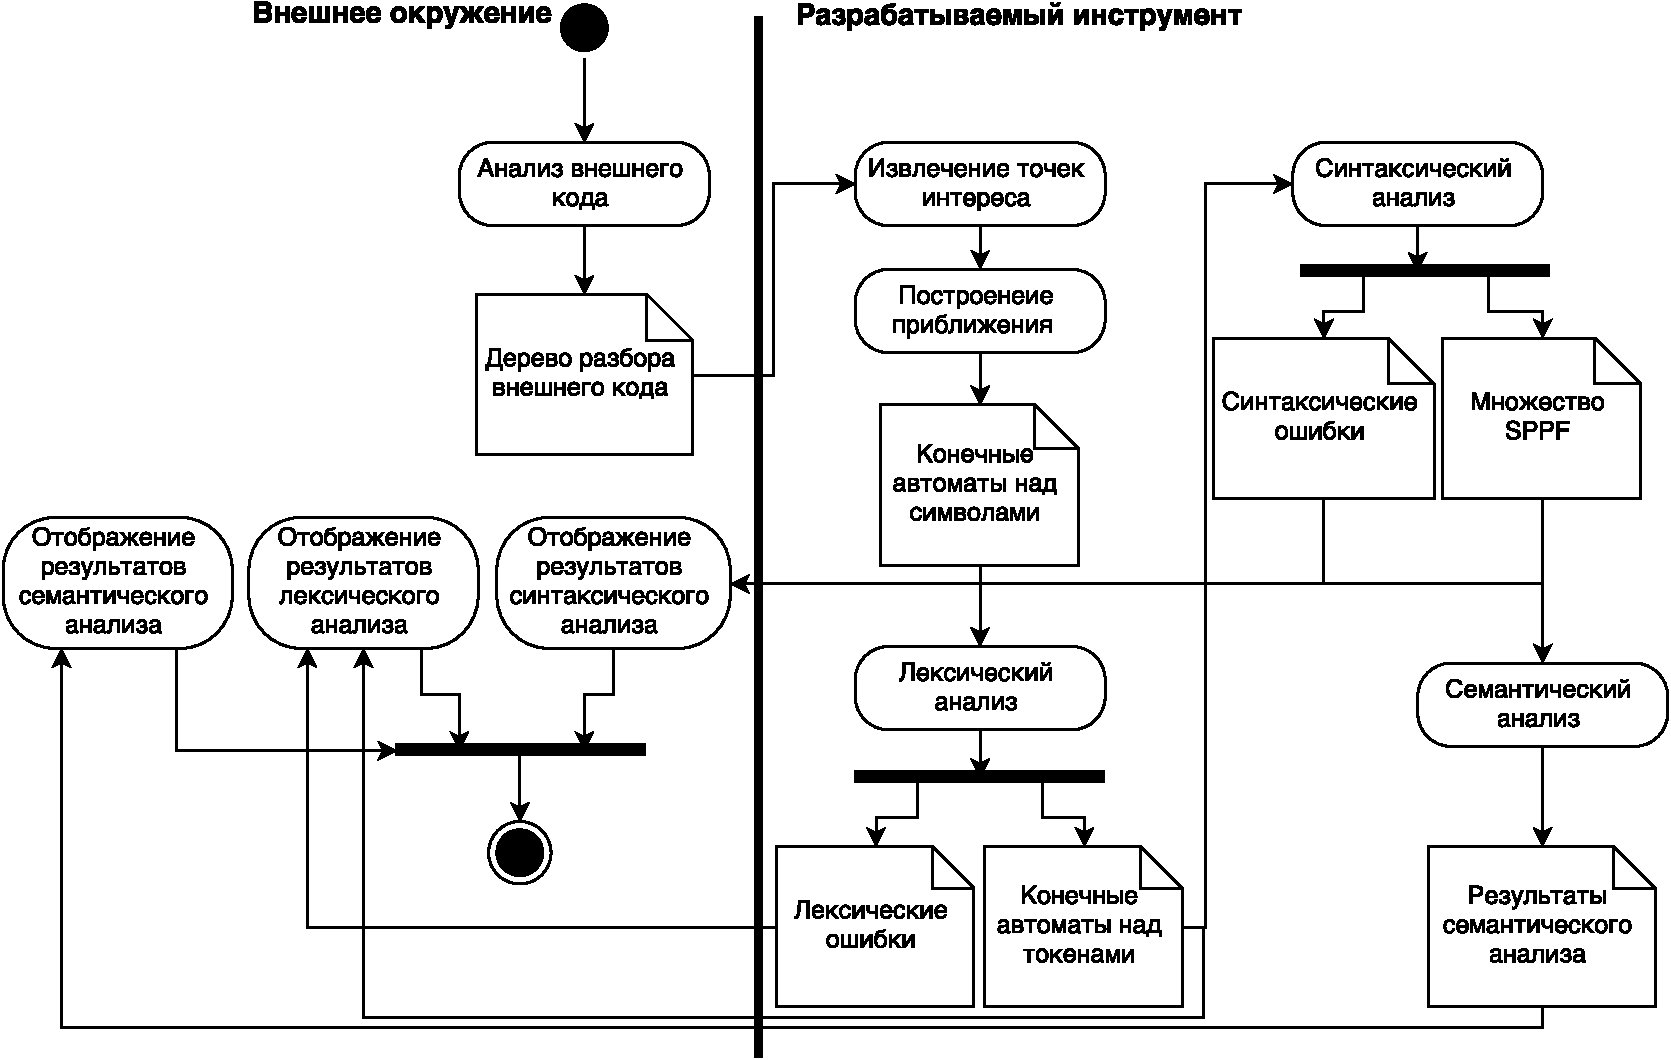
\includegraphics[width=0.95\textwidth]{Activ_SEL_Processing}
 \caption{Пороцесс обработки динамически формируемых выражений}
 \label{sel_processing}
\end{figure}


В \underline{\textbf{четвёртой главе}} описывается метод реинжиниринга встроенного программного кода, основные шаги которого представлены на рисунке~\ref{fig:method}. Данный метод позволяет сформулировать требования к конкретным инструментам обработки встроенного программного кода, необходимым для обработки конкретной информационной системы.

\begin{figure}[]
\begin{center}
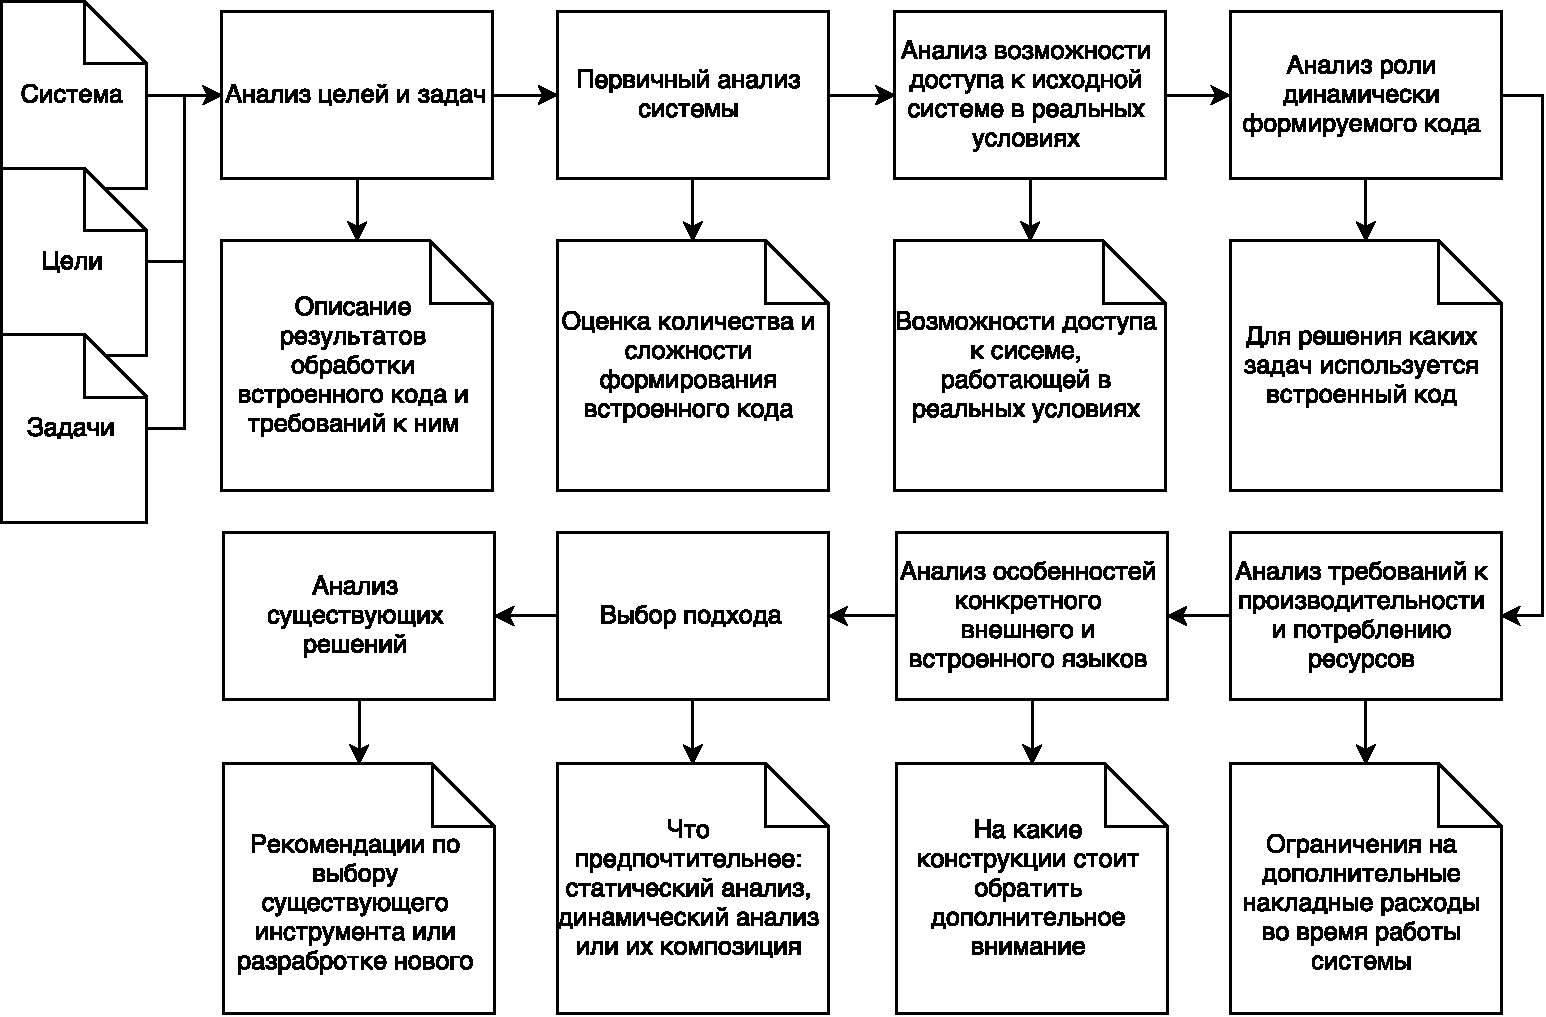
\includegraphics[angle=90,origin=c,width=.95\textwidth]{ReengMethodSteps}
\caption{Основные шаги метода обработки встроенных языков и их результаты}
\label{fig:method} 
\end{center}
\end{figure}


В \underline{\textbf{пятой главе}} приводятся результаты экспериментального исследования YC.SEL.SDK.

Реализованный инструментарий был апробирован в рамках промышленного проекта по миграции базы данных с MS-SQL Server 2005 на Oraclе 11gR2, что позволило оценить предложенную архитектуру и протестировать отдельные компоненты инструментария на реальных данных.

Обрабатываемая система состояла из 850 хранимых процедур и содержала около 2,6 миллионов строк кода. В ней присутствовало 2430 точек выполнения динамических запросов, 75\% этих запросов могли принимать 
более одного значения, при их формировании использовалось от 7 до 212 операторов, среднее количество операторов для формирования запроса равнялось 40.

Алгоритм успешно завершил работу на 2188 входных графах из 2430, аппроксимирующих множества значений запросов. Ручная проверка входных графов, на которых алгоритм завершался с ошибкой, показала, что они действительно не содержали ни одного выражения, корректного в эталонном языке. Причиной этого была либо некорректная работа лексического анализатора, либо наличие в выражениях конструкций, не поддержанных в существующей грамматике. Так как лексический анализатор и грамматика были полностью заимствованы из оригинального проекта, то наличие этих ошибок не является недоработками алгоритма синтаксического анализа. В дальнейшем часть найденых ошибок была исправлена.

Общее время синтаксического анализа составило 27 минут, из них 13 минут было затрачено на разбор графов, не содержащих ни одного корректного выражения, и 4 минуты на обработку графа, прерванную по таймауту. На анализ двух графов было затрачено более 2 минут. Распределение входных графов по интервалам времени, затраченным на анализ, приведено на рисунке~\ref{distr}.

\begin{figure}[]
  \centering
 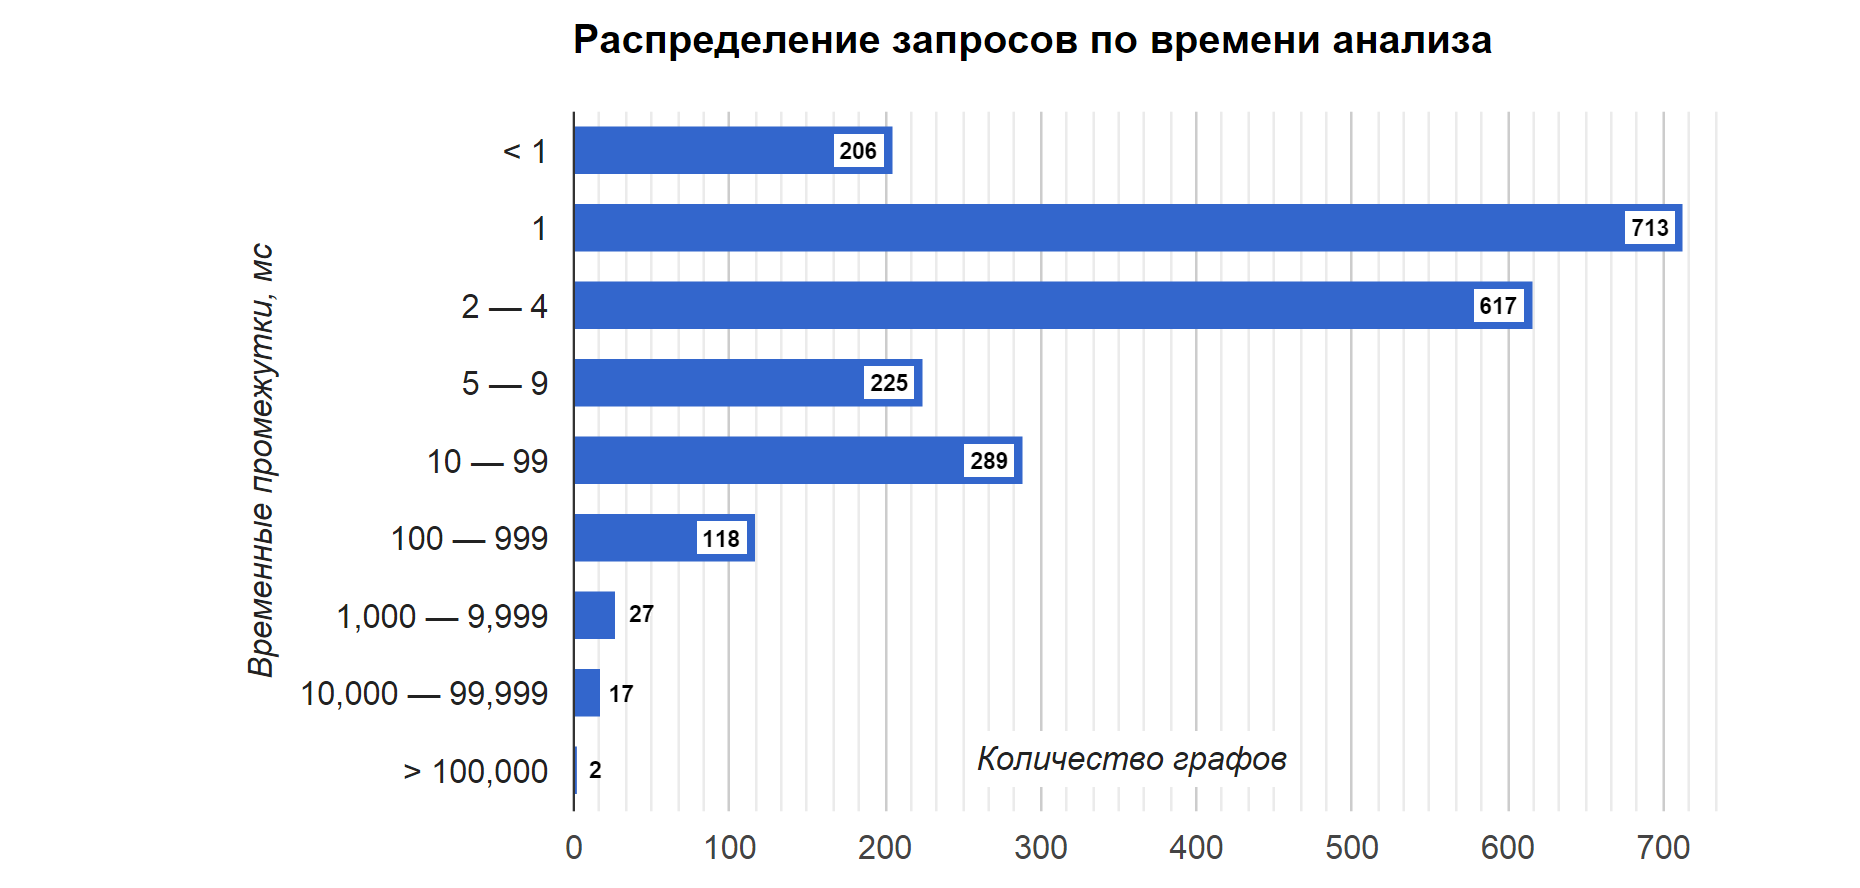
\includegraphics[width=0.95\textwidth]{distr.png}
 \caption{Распределение запросов по времени анализа}
 \label{distr}
\end{figure}


Также было проведено сравнение производительности компоненты синтаксического анализа YC.SEL.SDK с инструментом Alvor. Данный инструмент реализует подход, близкий к представленному в работе --- независимые шаги анализа, --- что позволяет легко выделить синтаксический анализ, который основан на GLR-алгоритме. Существенным отличием является то, что Alvor не строит деревьев вывода. Важным для успешного проведения измерений является то, что исходный код Alvor опубликован, что позволяет модифицировать его таким образом, чтобы измерять параметры выполнения конкретных методов. 

Так как Alvor не предоставляет платформы для простой реализации поддержки новых языков, то для сравнения было выбрано подмножество языка SQL, общее для Alvor и реализованного в рамках апробации инструмента. 
Измерения проводились на синтетических данных, построенных с помощью последовательного соединения базовых блоков, каждый из которых содержит ветвления с $h$ параллельными путями. Результаты экспериментов 
представлены на графике~\ref{fig:YCvsAlvor}. При более чем шестнадцатикратном повторении блоков с $h=2$ время работы Alvor превысило 30 минут и измерения были прекращены. Аналогичная ситуация возникает и при 
более чем десятикратном повторении блоков с $h=3$. Таким образом, измерения показывают, что время работы анализатора Alvor растёт экспоненциально относительно количества повторений базового блока при $h>1$. 
Анализатор созданный на основе YC.SEL.SDK в таких случаях имеет лучшую производительность. При этом на линейном входе Alvor работает быстрее. Однако существуют возможности для оптимизации текущей реализации, благодаря чему производительность на линейном входе может быть улучшена.

В результате сравнения было установлено, что на линейном входе Alvor показывает лучшую производительность, однако на входных данных, содержащих большое количество ветвлений и циклов производительность Alvor существенно хуже (до 1000 раз).

\begin{figure}[]
 \centering
 \includegraphics[width=0.95\textwidth]{AlvorVsYCbw.eps}
 \caption{Сравнение производительности Alvor и синтаксического анализатора на базе YC.SEL.SDK}
 \label{fig:YCvsAlvor}
\end{figure}

\underline{\textbf{Шестая глава}} содержит итоги сравнения и соотнесения полученных результатов с существующими аналогами. Получены следующие выводы.
\begin{enumerate}
    \item Разработанный алгоритм синтаксического анализа динамически формируемых выражений является единственным алгоритмом, обрабатывающим регулярную аппроксимацию, строящим конечное представление леса разбора.
    \item Созданная архитектура позволяет предоставить первую платформу для разработки средств анаиза динамически формируемого кода.
    \item Метод реинжиниринга встроенного программного кода сформулирован впервые.
\end{enumerate}



В \underline{\textbf{заключении}} подведены итоги диссертационной работы, сформулированы рекомендации по применению результатов работы в индустрии и научных исследованиях, а также сформулированы перспективы дальнейшей разработки представленной в работе тематики.

\newpage
\renewcommand{\refname}{\Large Публикации автора по теме диссертации}

\begin{thebibliography}{99}

\bibitem{1} Григорьев, С. В. Разработка синтаксических анализаторов в проектах по автоматизированному реинжинирингу информационных систем / Я. А. Кириленко, С. В. Григорьев, Д. А. Авдюхин // Научно-технические ведомости Санкт-Петербургского государственного политехнического университета информатика, телекоммуникации, управление. ---~2013. ---~Т.~3, \textnumero~174. ---~C.~94--98.
\bibitem{2} Григорьев, С. В. Инструментальная поддержка встроенных языков в интегрированных средах разработки / С. В. Григорьев, Е. А. Вербицкая, М. И. Полубелова и др. // Моделирование и анализ информационных систем. ---~2014. ---~Т.~21, \textnumero~6.  ---~С.~131--143.
\bibitem{3} Григорьев, С. В. Обобщенный табличный LL-анализ / С. В. Григорьев, А. К. Рагозина // Системы и средства информатики. ---~2015. ---~Т.~25, \textnumero~1.  ---~С. 89--107. 

\bibitem{4} Grigorev, S. GLR-based abstract parsing / S. Grigorev, I. Kirilenko // In Proceedings of the 9th Central \& Eastern European Software Engineering Conference in Russia (CEE-SECR ’13). ---~2013. ---~P.~1--9.
\bibitem{5} Grigorev, S. String-embedded language support in integrated development environment / S. Grigorev, E. Verbitskaia, A. Ivanov et al. // Proceedings of the 10th Central and Eastern European Software Engineering Conference in Russia (CEE-SECR '14). ---~2014. ---~P.~1--11.
\bibitem{6} Grigorev, S. From Abstract Parsing to Abstract Translation / S. Grigorev, I. Kirilenko // Proceedings of the Spring/Summer Young Researchers' Colloquium on Software Engineering. ---~2014. ---~P.~1--5.
\bibitem{7} Grigorev, S. Relaxed Parsing of Regular Approximations of String-Embedded Languages / E. Verbitskaia, S. Grigorev, D. Avdyukhin // Preliminary Proceedings of the PSI 2015: 10th International Andrei Ershov Memorial Conference. ---~2015. ---~P.~1--12.

\end{thebibliography}
